\cleardoublepage
\chapter{Introduction}
\label{intro}
%\markboth{Introduction}{Introduction}
%\addcontentsline{toc}{chapter}{Introduction}
%A non-numbered chapter\dots

\section{Motivation}
\label{intro_motivation}

% Potential re-formulation
%Paragraph 1: Energy transition, Paris agreement
% Paragraph 2: Covid-19 pandemic and focus on cities
% Paragraph 3: Spatial and temporal estimation, Increasing data availability
% Paragraph 4: Research gap addressed in the thesis
% Paragraph 5: Switzerland and urban environment as focus
% SOURCE: Research plan

The decarbonisation of the energy system plays an important role in fulfilling the ambitious emission targets set by the Paris Agreement, which aims to limit global warming to well below 2$^\circ$C below pre-industrial levels \cite{rogelj_paris_2016}.
To contribute to achieving this goal, governments around the world have established national energy policies, setting targets for the use of renewable energies (RE) within the next 10 - 30 years. 
\nomenclature[A]{RE}{Renewable energy}
An analysis of worldwide RE policies~\cite{ren21_renewables_2020} showed that in 2019, 166 countries had specific targets for shares of renewable electricity production, while only only 49 countries have established targets for the heating and cooling sector, of which very few reach beyond 2020. 
As a consequence, roughly 26\% of current electricity production is provided through RE, while only 10\% of heating and cooling energy is provided renewably. However, heating and cooling makes up more than half of the worldwide final energy consumption (in 2017, see Fig. \ref{fig:ren21_RE_use}). These numbers call for an increased focus on decarbonisation targets for the heating and cooling sectors, in particular through cross-sectoral policies  \cite{ren21_renewables_2020}.
% BRING IN HYBRID

\begin{figure}
\centering 
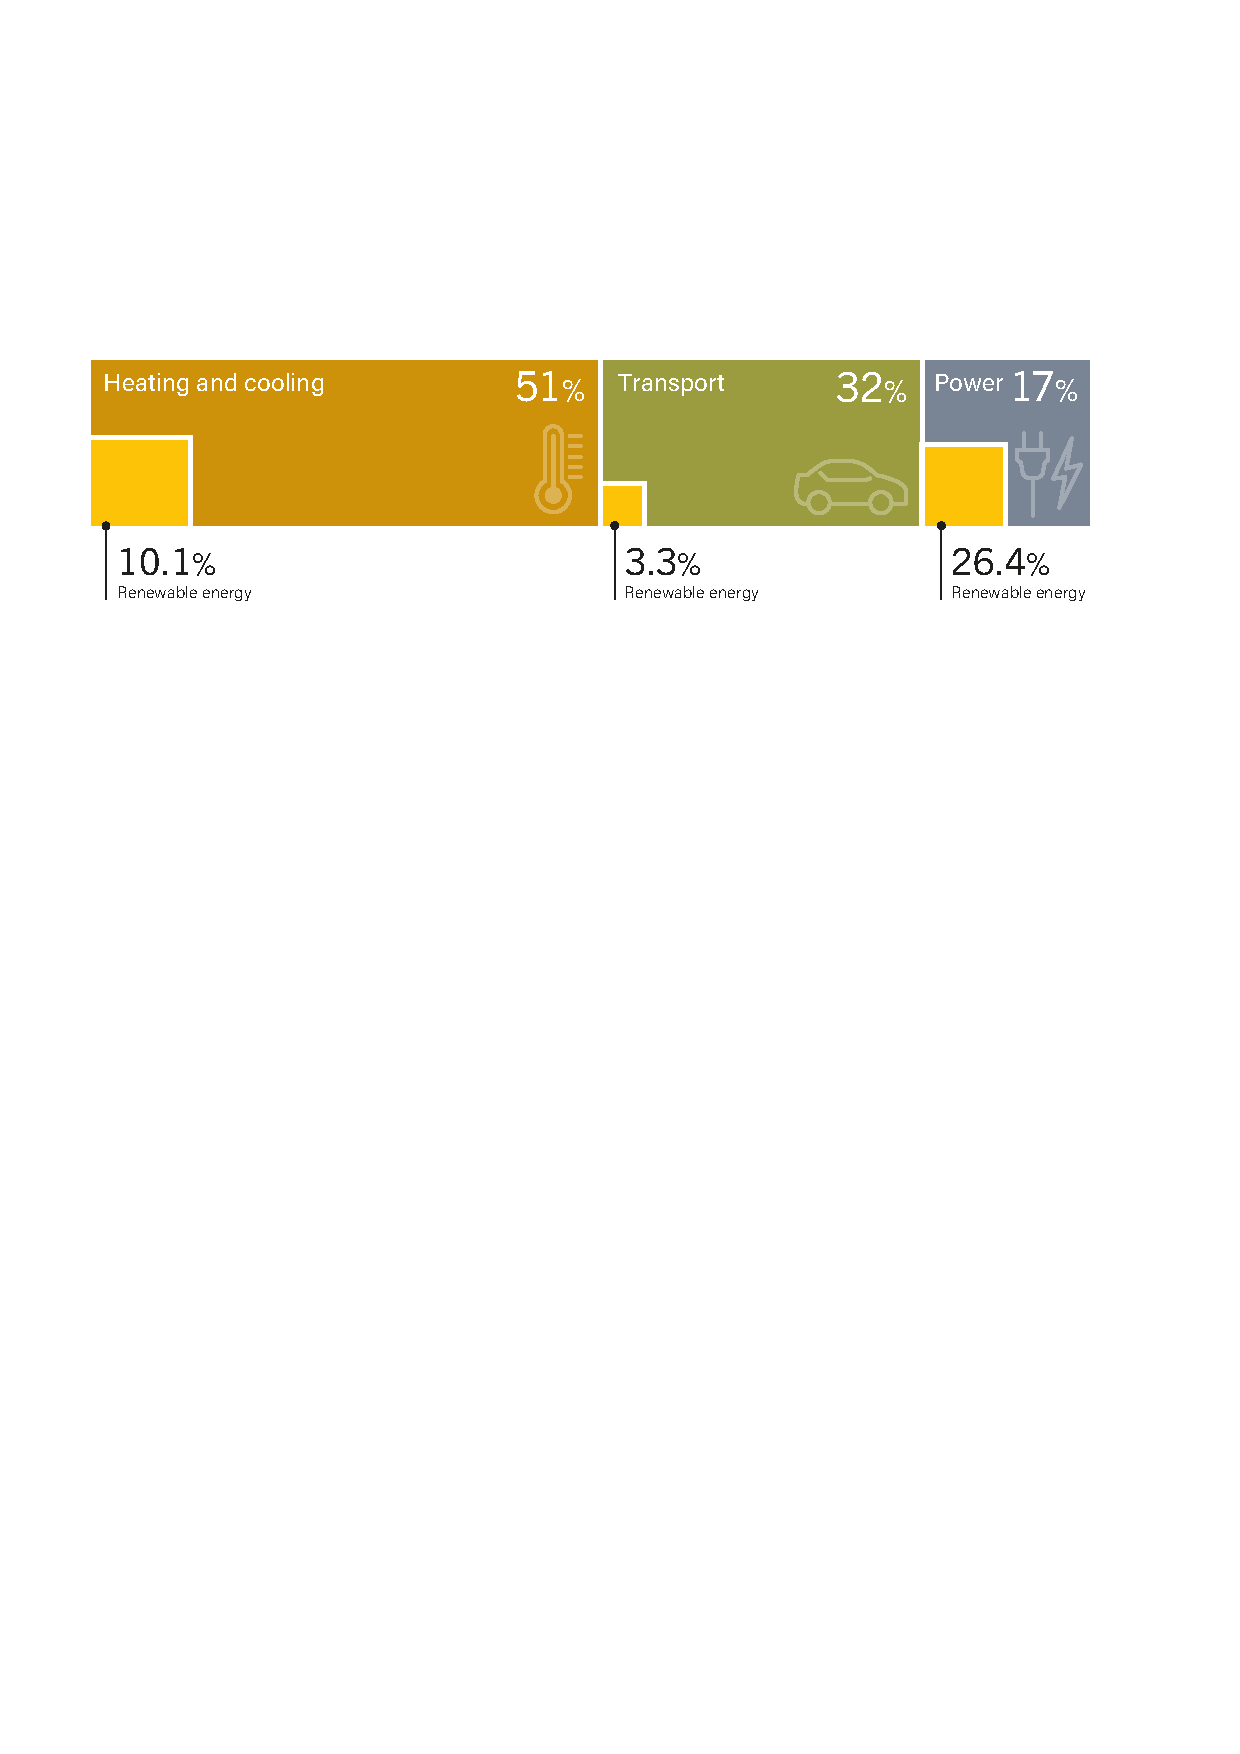
\includegraphics[width=\textwidth]{images/gsr_2020_RE_share.pdf} 
\caption[Renewable Share of Total Final Energy Consumption, by Final Energy Use, 2017]{Renewable Share of Total Final Energy Consumption, by Final Energy Use, 2017. Source: \citet{ren21_renewables_2020} (Based on IEA data)}
\label{fig:ren21_RE_use} 
\end{figure}

In this context, global energy reports highlight the current Covid-19 pandemic as a crucial opportunity to push towards more ambitious RE strategies \cite{iea_world_2020,irena_global_2020,fs-unep_global_2020}. 
The disruption to the energy sector caused by the pandemic exceed any event in history, and the consequences will last for years \cite{iea_world_2020}. 
As governments all around the world are developing huge recovery packages to support their societies and economies, aligning these packages with the medium and long-term goals of the Paris Agreement may lead to a "shift to sustainable, decarbonised economies and resilient inclusive societies" \cite{irena_global_2020}. 
The potential RE generation in urban environments is hereby of high interest, as cities are responsible for a large share of current global greenhouse gas emissions and are expected to host two thirds of the world population by 2050 \cite{irena_rise_2020}. 

Developing effective national and regional strategies to integrate RE into future energy systems requires knowledge of the potential energy generation from the available renewable resources. 
This includes information on \textit{which} technologies may provide a significant amount of energy, \textit{where} RE resources may be exploited and \textit{when} they are available. 
These aspects may be assessed through spatio-temporal modelling, which characterises both the spatial (\textit{"where"}) and temporal (\textit{"when"}) patterns of the energy generation from given RE resource.
The spatio-temporal modelling of RE potentials is however dependent on the availability of sufficient and high-quality data on the natural resources and the environment.
Rapid improvements in the quantity and quality of data collected at national and global levels, for example through satellite imagery, weather stations and land surveys, as well as in computational methods for data handling and analysis allows to assess these potentials in unprecedented ways.

% Paragraph: Switzerland
% Currently, there is no methodology that estimates the large-scale RPV potential at a high spatio-temporal resolution and also addresses the systematic propagation of uncertainties arising from the modelling process.
% This paper contributes to fill this gap by adapting state of the art methods for the assessment of RPV potential in order to quantify and combine different sources of uncertainty. 
% We further use Machine Learning to incorporate information that is only available in parts of the study region of Switzerland.
Motivated by the need for cross-sectoral RE policies, the push for RE incentives as part of  Covid-19-related recovery strategies and the opportunities presented through an increasing amount of energy-related data, this thesis aims to estimate a \textit{hybrid renewable energy potential} (HyREP) for the built environment at national scale. 
\nomenclature[A]{HyREP}{Hybrid Renewable Energy Potential}
The HyREP describes the spatial and temporal patterns of several renewable energy resources for electricity \textit{and} heat generation, which may be combined with other (non)-renewable energy sources to assess potential complementarities between energy sources and their potential for satisfying the energy demand of cities. 

% something about a database, focus on methodological aspects to have a spatially comparable potential, as well as establishing database
This thesis focuses on RE potential within the built environment, since the built environment gives rise to a large amount of the national electricity and heat demand. Directly satisfying this demand where it occurs reduces the need for heat and power transmission over large distances, which reduces losses and can help to reduce supply peaks due to the intermittency of RE resources. 
The focus of the work lies in the spatio-temporal estimation of the technical potential of RE sources at large scale, whereby the technical potential is defined as the maximum energy (heat or electricity) which can be provided using a specific RE technology. 
These resource potentials include physical, geographical and technical limitations and yield results at the scale of individual building or property units, at hourly or monthly temporal resolution for a large geographic area, such as the country of Switzerland. 

We assess the potential energy generation from two renewable resources which have been growing rapidly in Switzerland, namely rooftop solar photovoltaics (RPV) and ground-source heat pumps (GSHPs), which extract shallow geothermal heat at depths of < 400 m. 
The resource assessments form publicly available databases of RE potential, which can be used to study hybrid systems from neighbourhood to country scale based on data that is homogeneous across the country. 
By combining state-of-the-art analytical models of RE technologies with large-scale data processing techniques and advanced statistical methods, including Machine Learning (ML), the HyREP datasets presented in this thesis contain a high level of detail on the natural resources, the built environment and the modelled technologies.
\nomenclature[A]{ML}{Machine Learning}
To demonstrate how the renewable energy databases can be used for the study of hybrid energy systems (HES), this thesis concludes with an analysis of the potential self-coverage and self-sufficiency of urban neighbourhoods across the country through the large-scale deployment of RPV and GSHPs, setting these results in context with the Swiss Energy Strategy for 2050.
\nomenclature[A]{HES}{Hybrid Energy System}
\nomenclature[A]{RPV}{Rooftop PV}

% More specifically, the potential energy generation from two renewable resources is assessed, namely solar and geothermal energy. 
% The potential includes electricity and heat generation from rooftop-mounted solar photovoltaics (PV) and solar thermal collectors (STC), respectively, and heat generation from shallow (<400m) geothermal energy using borehole heat exchangers (BHE). 

% While to date individual aspects have been studied at national scale, no large-scale approach exists to model hybrid potential at high temporal and high spatial resolution to quantify the geographic distribution of storage requirements and maximum energy mismatch. Assessing for the first time the spatio-temporal distribution of hybrid energy potential on national scale can hence give a comprehensive view on the opportunities and risks of hybrid systems and on the regional and national energy balance. 

% Focusing on the Swiss energy landscape, this research aims to quantify the potential for distributed hybrid energy generation using state-of-the-art data-driven methods.

% END WITH SWITZERLAND

% INTERSECTION OF DATA-DRIVEN AND PHYSICS-BASED MODELS

\section{A hybrid renewable energy potential for Switzerland}
\label{intro_REN}


Estimation of a hybrid renewable energy potential for Switzerland requires answering the following questions: 
\begin{itemize}
\item Which renewable energy resources are available in Switzerland?
\item How can the potential of these resources be spatially and temporally estimated?
\item What defines a hybrid renewable energy potential?
\end{itemize}

\subsection{Renewable energy in Switzerland}
\label{REN_CH}

Two types of renewable energies (RE) will be investigated in this study: solar energy and geothermal energy. These energies are amongst the fastest-growing RE in Switzerland in the last 10 years [1], with growth rates shown in Figure 1. Throughout this study, rooftop-mounted solar installations will be considered for electricity generation from photovoltaic (PV) panels, as well as for heat production for domestic heating and hot water applications from thermal collectors. Geothermal heat generation potential will be calculated for shallow depth (up to 400m) in accordance with current standards for domestic applications. Note that geothermal electricity generation is not considered as this technology is not applied in the domestic sector [2]. 

\begin{figure}[tb] 
\centering 
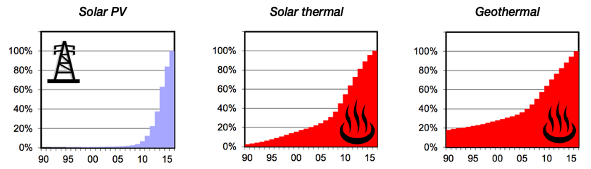
\includegraphics[width=\textwidth]{REN_CH} 
\caption[Growth rates of solar PV, solar thermal and geothermal technology application in Switzerland in the past 25 years.]{Growth rates of solar PV, solar thermal and geothermal technology application in Switzerland in the past 25 years. The data is given in \% of production for 2016 [1].}
\label{fig:ren_ch} 
\end{figure}

\subsubsection{Solar energy from photovoltaics and thermal collectors.}
As solar energy is abundantly available and easy to harvest, solar PV and solar thermal technologies have attracted worldwide interest. Most studies of solar potentials focus on PV potentials, for example in Switzerland [3]–[5], USA [6], Spain [7], [8], Germany [9], [10]. Solar thermal potentials on the large scale are rarely quantified; this may be partly due to a lower interest in solar thermal collectors for residential applications [1] and partly due to the high interdependency between collector efficiency and heat demand [11]. Large-scale potential studies have been carried out for thermal power plants in India [12], and for residential buildings in Switzerland [11]. Potentials are typically computed as monthly or yearly values; there is however no current study estimating the large-scale potential at an hourly timescale, which is necessary to quantify a potential for hybrid energy systems and requirements for energy storage. 

\subsubsection{Shallow geothermal energy from borehole heat exchangers}
Geothermal energy is equally abundant as solar energy, as it accesses heat from the earth’s core. However, accessing this resource is more complex, as it requires drilling into the ground. In Switzerland, 95\% of geothermal installations are ground-source heat pump (GSHP) systems. Several GSHP technologies exist to access shallow geothermal energy in the built environment, some of which are shown in Figure 4. The most frequently used technology are borehole heat exchangers (85\% of GSHP in Switzerland), followed by ground water wells (13\%) \cite{blum_statistik_2016}. Very shallow technologies (up to 10m), despite being easy to place, are currently not widely used because of large space requirements and lower efficiency due to seasonal variation of ground temperature at low depth. The highest interest for this study lies thus in the calculation of shallow geothermal potentials at depths of 100-200m, which are typical depths of BHEs in Europe \cite{rybach_design_2014}.

\begin{figure}
\centering 
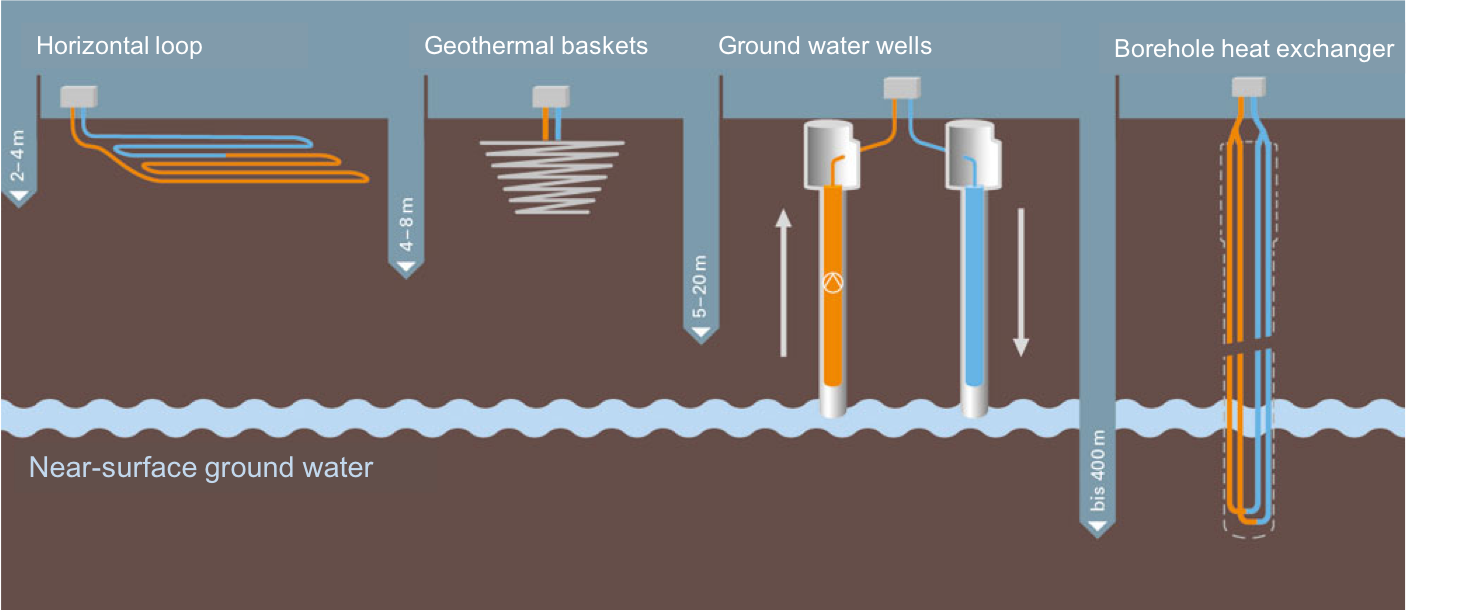
\includegraphics[width=\textwidth]{images/Figs/shallow_technologies.png} 
\caption{Key technologies for near-surface geothermal installations (up to 400m) \cite{noauthor_arten_nodate}.}
\label{fig:shallow_gshp} 
\end{figure}

\subsection{Spatio-temporal estimation of renewable energy potentials}

%% SOURCE: Research plan
For the computation of large-scale solar energy potentials, related studies widely apply a hierarchical approach [3], [4], [7], [13], illustrated in Figure 2. The first step is the calculation of a physical or theoretical potential, which represents the amount of energy that natural resources in the region of interest can provide (per unit area). In the second step, the geographic or urban potential is calculated, which accounts for the impact of the built environment on the natural resources. It measures the amount of energy that can be collected by the panels or collectors. The third step gives the technical potential and accounts for losses during conversion of the natural resources to domestic heat and electricity. It gives the maximum feasible amount of energy that can be harvested using a given technology. After obtaining the maximum feasible energy output, one may consider additional environmental, economic or social considerations to refine the estimated size of the system. A fourth step may thus be an economic potential focused on sizing the systems under given constraints. Economic considerations such as technology cost are not taken into account in the reviewed large-scale studies. Instead, they have been assessed in separate studies, in smaller-scale case studies as well as in hybrid potential assessments. An analysis of market potential is beyond the scope of this work. 
 
% Figure 2: Hierarchical approach for estimating rooftop PV and solar thermal potentials. [14]

\subsection{Definition of hybrid renewable energy potential}

\section{Research aims and objectives}
\label{intro_goals}
% SOURCE: Research plan
The main driver behind this study is the question whether it is possible to cover urban energy demand in Switzerland using a combination of renewable energies, and which level of energy autonomy could be reached in the built environment from this hybrid renewable energy potential. Special interest lies hereby on the spatial and temporal variability of the supply in order to match the seasonal and intra-day variations of the energy demand. With the focus on two types of resources, solar and geothermal energy, the following research questions arise:

\begin{itemize}
\item How can the potential for renewable energy resources in the built environment be estimated on national scale for Switzerland, and what are the related uncertainties?
\item What impact does the combination of multiple renewable resources to hybrid systems have on distributed energy supply?
\item How can data-driven methods and Machine Learning be applied to improve current ways of estimating potential and to facilitate their scalability to national scale?
\end{itemize}

The above questions have been partly addressed in case studies on building and district scale, or as large-scale studies of individual aspects, but no unified approach exists to assess hybrid energy potential for the built environment at high spatial and temporal resolution. Large-scale potential assessment has been performed in most cases in monthly resolution only, or without considering any spatial distribution of potentials. Many case studies have been conducted, but most models are computationally intensive and infeasible for application the large scale. Furthermore, a comprehensive analysis of uncertainties related to estimation and modelling is rarely provided. Machine Learning has been used in some studies, but there is still a huge potential that can be exploited to understand patterns in the available resources, approximate missing data and model system behaviour in a more computationally efficient way.

This study aims to combine methodologies of large-scale potential assessment and small-scale system modelling to quantify hybrid energy potential in the built environment for Switzerland. Data-driven methods and Machine Learning will be used to overcome gaps caused by lack of data and computational efficiency. The proposed assessment will make use of a large variety of environmental data and will present a unified approach that allows to compare the potential of some of the most promising renewable resources in the built environment. These resources will be combined with the energy demand to derive a hybrid potential which complements the demand patterns. The research hypothesis is hereby that hybrid systems in the built environment bring advantages over single-technology systems, and that a significant fraction of the energy demand can be covered by hybrid renewable potential if the energy mix is chosen appropriately.

The study is divided in three phases. The first phase focuses on electricity. It is divided into the computation of hourly solar energy potentials (WP1) and the assessment of hybrid electricity potential based on solar PV and wind energy (WP2). The second phase focuses on heat energy. In this phase, geothermal energy potentials will be evaluated (WP3) and combined with solar thermal potentials to a hybrid heat potential (WP4). A case study for a selected district will be conducted to assess multi-energy potentials and their effect on covering the urban energy demand. Finally, visualization methods for multi-dimensional data will be explored. 

% SOURCE: Research plan 
% The first phase of the study focuses primarily on electricity, i.e. the estimation of solar PV potential and its combination with electricity generation from wind and electricity demand (external inputs). During the second phase, heat systems with geothermal and solar thermal heat generation will be investigated. For the computation of potentials, data-driven modelling using Machine Learning algorithms is combined with parallelisation of analytical models to cope with the high spatial and temporal resolution of the relevant datasets. Geographic information systems (GIS) are further used to handle geographically referenced datasets. Efforts are made to quantify the uncertainty related to several modelling steps throughout the study and to identify the sources of uncertainties, for example caused by modelling or by data noise.

\section{Structure of the thesis}
To address the above research goals, the thesis is structured as follows:

\textbf{Part~\ref{methods}} provides a summary of state-of-the-art analytical and statistical methods used in the thesis and large-scale datasets used in the national REN potential studies. \textbf{Chapter~\ref{methods_physical}} introduces analytical methods for modelling physical processes and technological aspects of RPV and GSHP systems. \textbf{Chapter~\ref{methods_ML}} covers Machine Learning methods used in this work and stastical approaches for uncertainty estimation.  \textbf{Chapter~\ref{data}} provides an overview over the available meteorological, environmental and building-related datasets for Switzerland.

\textbf{Part~\ref{potential} }addresses the estimation of renewable energy potentials. \textbf{Chapter~\ref{solar} } details the developed model for estimating rooftop solar photovoltaic potential at national scale, as well as a  comparison of the resulting potential database with existing estimations for Switzerland. \textbf{Chapter~\ref{geothermal}} provides the estimation of technical potential for shallow geothermal energy, using analytical models at regional scale and Machine Learning for the estimation at national scale. The chapter further shows an approach to expand the model to include thermal regeneration of the geothermal resources through cooling re-injection to the ground with regional-scale application.

\textbf{Part~\ref{hybrid}} demonstrates the application of the potential databases developed in Part~\ref{potential} for modelling hybrid renewable energy systems. \textbf{Chapter~\ref{hybrid_chapter}} outlines a mapping approach for the energy demand of heat and electricity from readily available data, which is a necessary complementary input to perform hybrid system studies. [TO BE CONTINUED].

\textbf{Chapter~\ref{conclusion}} concludes with the main findings of the thesis and a future outlook.



